\begin{frame}{Beschreibung}{Dokument-Management-Zyklus}
\begin{figure}
\centering
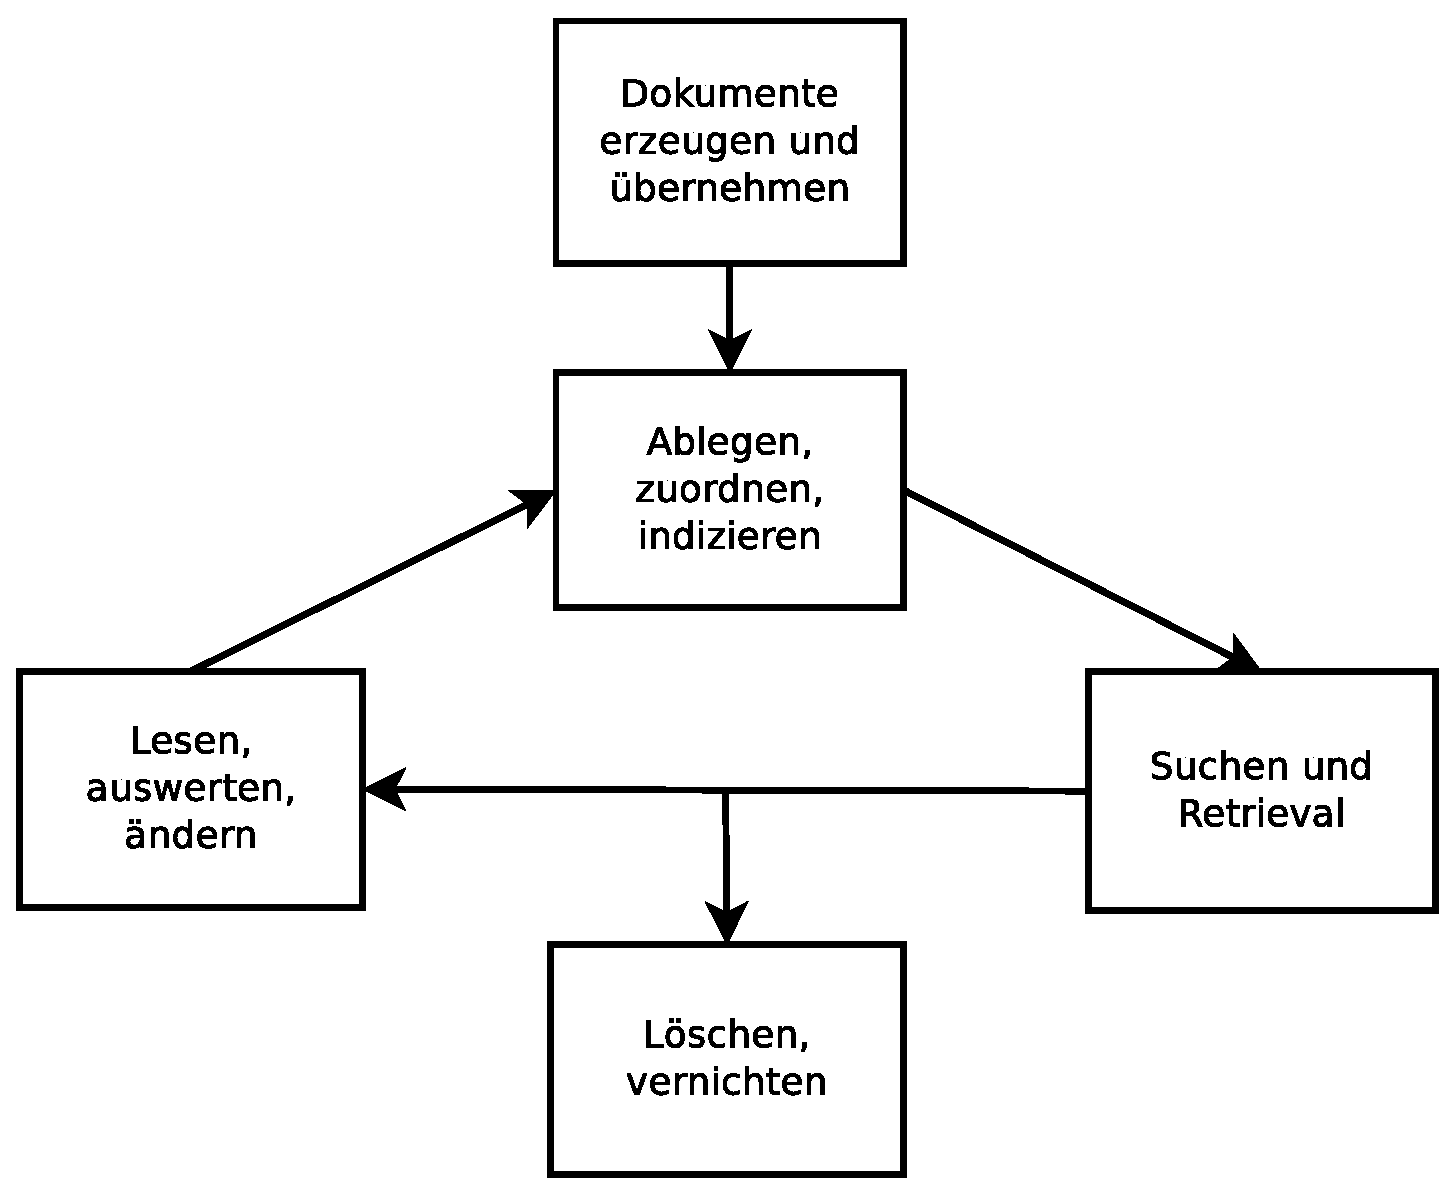
\includegraphics[width=.5\linewidth]{images/Dokumenten-Management-Zyklus}
\caption[Dokumenten-Managemente-Zyklus]{Der Dokumenten-Management-Zyklus \cite{Götzer2014}}
\label{dmk}
\note<1>
{
	\begin{itemize}
		\item Einbindung mit Office-Software, Importierungsfunktionen (Digitalisieren/Scannen/Fax)
		\item Archivierung, Metadaten, Schlagwörter/Tags
		\item nach Keywords, Inhalt (OCR) suchen
		\item Sensitive Daten Vernichten (Verschlüsselung)
		\item Vorschau, Google-Docs Integration
	\end{itemize}
}
\end{figure}
\end{frame}